\documentclass[../../../thesis.tex]{subfiles}

\begin{document}
  \begin{figure}[bt]
		\centering
    \tikzsetnextfilename{kelvin_equation_plot}
    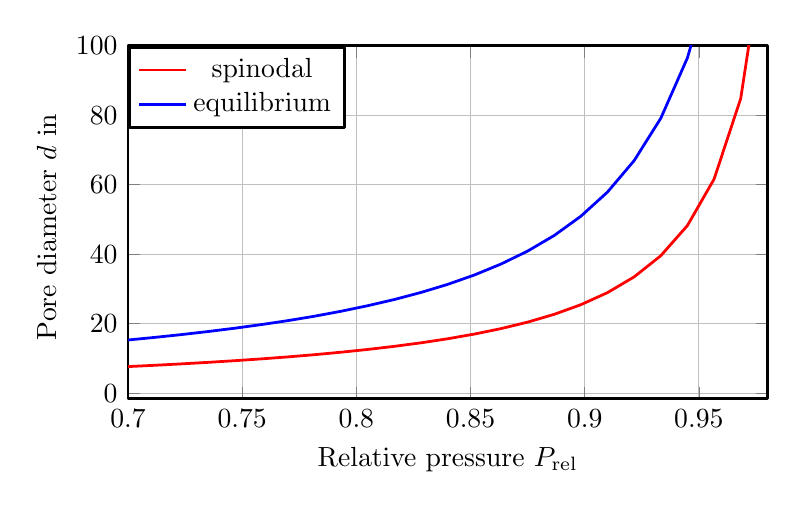
\begin{tikzpicture}
      \def\R{8.3144598}     %
      \def\gamma{0.018605}  % newton per meter
      \def\T{19+273.15} % kelvin
      \def\Vm{0.13053}  % litre per mol
        \begin{axis}[
          /tikz/line join=bevel,
          width=0.8*\textwidth,
          height=0.5*\textwidth,
          grid,
          legend style={at={(0,1)}, legend columns=1, anchor=north west},
          every axis plot,
					line width = 1pt,
					%	minor x tick num= ,
					%	minor y tick num= ,
					xmin = 0.7, xmax = 0.98,
					ymax = 100,
					xlabel = {Relative pressure $P_\mathrm{rel}$},
					ylabel = {Pore diameter $d$ in $\si{\nano\meter}$},
          ]
            \addplot[domain=0.7:0.98, red]
              {- (2 * \gamma * \Vm / \R / \T / 100 ) / ln(x)};
            \addlegendentry{spinodal}
            \addplot[domain=0.7:0.98, blue]
              {- 2*(2 * \gamma * \Vm / \R / \T / 100 ) / ln(x)};
            \addlegendentry{equilibrium}
          \end{axis}
    \end{tikzpicture}
    \caption{Pressure to diameter conversion by \textsc{Kelvin} equation for the parameters $T=\SI{19}{\celsius}$, $\gamma_\mathrm{T=\SI{19}{\celsius}}^\mathrm{hexane} =\SI{0,018605}{\newton\per\meter}$ and $V_\mathrm{mol,T=\SI{19}{\celsius}}^\mathrm{hexane}=\SI{0.13053}{\liter\per\mol}$.}
    \label{fig:kelvin-equation-plot}
  \end{figure}
\end{document}
